\documentclass{report}
\usepackage[utf8]{inputenc}
\usepackage[francais]{babel}  
\usepackage[T1]{fontenc} 
\usepackage{graphicx}
\usepackage{listings}
\renewcommand{\thesection}{\arabic{section}}
\begin{document}

\section*{Optimisation du Code}
\subsection*{La division}

L'opération la plus lognue dans notre kernel est la division. A chaque exécution du kernel, celle-ci est éxécutée $n^2$ fois.

On inverse les boucles, ainsi on ne fait plus que $n$ divisions ; mais on doit faire en plus $n^2$ multiplications par appel du kernel.
\\Sur les processeurs Ivy Bridge, la multiplication est environ 3$\times$ plus rapide que la divsion. En considérant qu'une multiplication est faite en 1 cycle, on peut donc comparer.
Sans les boucles inversées,le traitement fait $n^2$ divsions, pour une durée de $3n^2$.
Avec les boucles inversées,le traitement fait $n$ divisions et $n^2$ multiplications, soit une durée de $3n+n^2$.
On compare $3n^2$ et $3n+n^2$:\\
\begin{figure}[ht!]
    \centering
    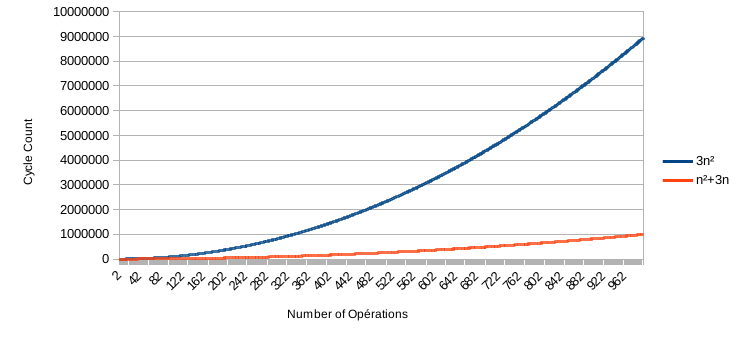
\includegraphics[width=100mm]{MEDIA/div_vs_mult_graph.png}
    \caption{Comparaison des temps de calcul des deux méthodes}
\end{figure}
Inverser les boucles est donc beaucoup plus rentable.



\end{document}
